\documentclass[doktyp=semarbeit, sprache=german]{TUBAFarbeiten}
\usepackage[utf8]{inputenc}
\usepackage[T1]{fontenc}
\usepackage{graphicx} 
\usepackage{amsmath}
\usepackage{subcaption}
\usepackage{booktabs}
\usepackage{url}
\usepackage{listings}
\lstset{
  language=bash,
  basicstyle=\ttfamily
}
\captionsetup{compatibility=false}
\bibliographystyle{unsrt}
\TUBAFFakultaet{Fakultät für Mathematik und Informatik}
\TUBAFInstitut{Institut für Informatik}
\TUBAFLehrstuhl{Lehrstuhl für Betriebssysteme und Kommunikationstechnologien}
\TUBAFTitel{Aufbau eines Prototyps für verteilte CUDA Programmierung}
\TUBAFUntertitel{Development of a prototype for distributed CUDA programming}
\TUBAFKorrektor{Dr. rer. nat. Martin Reinhardt}
\TUBAFBetreuer{Prof. Dr. Konrad Froitzheim}
\TUBAFAutor[S. Dressel]{Samuel Dressel}
\TUBAFStudiengang{Angewandte Informatik}
\TUBAFVertiefung{Parallelrechner}
\TUBAFMatrikel{59963}
\TUBAFDatum{\today}
\begin{document}
\maketitle
\tableofcontents
\TUBAFErklaerungsseite
\newpage
\section{Einleitung}
\section{Grundlagen}
\subsection{Message-Passing-Interface (MPI)}
Das Message-Passing-Interface, kurz MPI, ist eine standartisierte Schnittstelle für die Kommunikation zwischen verteilten Prozessen.
\subsection{CUDA-Aware MPI}
\section{Technischer Aufbau und Konfiguration}
Für den Aufbau des Mini-Clusters werden zunächst folgende Dinge benötigt:
\begin{itemize}
	\item Nvidia Jetson Nano (3x)
	\item SD-Karte (3x)
	\item Ethernet-Kabel (4x)
	\item 4-Port Ethernet Switch
	\item Optional: 40mm Lüfter (3x, in diesem Fall wurde der Noctua NF-A4x20 verwendet)
\end{itemize}
Der technische Aufbau beginnt mit der physischen Verbindung der Nvidia Jetson Nanos. Dazu werden diese alle via Ethernet-Kabel mit einem Ethernet Switch verbunden, welcher wiederum durch LAN mit einem Router und dadurch mit dem Internet verbunden ist. An sich benötigt der Cluster keinen Internetzugang, für die Einrichtung ist dieser jedoch unersetzlich. Einer der Jetson Nanos fungiert als Head-Node (Masterknoten), die anderen zwei als Worker-Nodes.
\\Ist das physische Setup abgeschlossen, wird als nächstes auf jedem der Jetson Nanos das Jetson Nano Developer Kit SD Card Image installiert. Dies geschieht durch das Schreiben des Images auf die jeweilige SD-Karte und einem anschließenden Setup auf den Jetson Nanos \cite{SDImage}. Danach wird das System durch Aktualisierung der Pakete auf den neuesten Stand gebracht:
\begin{lstlisting}
sudo apt-get update
sudo apt-get upgrade
\end{lstlisting}
Es folgt die Installation des \texttt{nano}-Texteditors und des SSH-Paketes. Dabei ist SSH für den Remotezugriff auf die einzelnen Knoten notwendig; an Stelle des \texttt{nano}-Texteditors kann alternativ jeder andere Editor benutzt werden.
\begin{lstlisting}
sudo apt-get install nano
sudo apt-get install openssh-server
\end{lstlisting}
Zusätzlich ist auf dem Masterknoten der NFS-Kernel-Server zu installieren:
\begin{lstlisting}
sudo apt-get install nfs-kernel-server
\end{lstlisting}
Auf den Worker-Nodes wird dagegen das \texttt{nfs-common}-Paket installiert:
\begin{lstlisting}
sudo apt-get install nfs-common
\end{lstlisting}
NFS und die damit verbundenen Pakete sind notwendig, um später Dateien innerhalb des Clusters auszutauschen.
\\Um dieses Netzwerk einzurichten, muss zunächst jedem der drei Knoten eine statische IP zugewiesen werden. Dies erfolgt entweder über die Netzwerkeinstellungen oder über das Bearbeiten der Interface-Datei:
\begin{lstlisting}
cd /etc/network
sudo nano interfaces
\end{lstlisting}
Dafür werden der Datei folgende Zeilen hinzugefügt:
\begin{lstlisting}
auto eth0
iface eth0 inet static
address 192.168.178.10
gateway 192.168.178.1
netmask 255.255.255.0
\end{lstlisting}
Dabei ist die Adresse \texttt{192.168.178.10} die Adresse des Masterknotens, die Worker-Nodes erhalten dann dementsprechend die IP-Adressen \texttt{192.168.178.11} und \texttt{192.168.178.12}. Damit die Änderungen wirksam werden, müssen entweder die Jetson Nanos oder der Network-Service neugestartet werden.
\\Als nächstes erfolgt die Einrichtung von SSH innerhalb des Clusters. Dazu wird zuerst jedem Knoten ein Name zur besseren Identifikation zugewiesen. Hierfür wird die \texttt{hostname}-Datei bearbeitet:
\begin{lstlisting}
sudo nano /etc/hostname
\end{lstlisting}
Der Masterknoten erhält in diesem Fall den Namen \texttt{master}, die Worker-Nodes die Namen \texttt{slave1} und \texttt{slave2}. Als nächstes werden in der \texttt{hosts}-Datei die statischen IP-Adressen aller Knoten hinzugefügt. Dies geschieht wie der vorige Schritt auf allen Knoten:
\begin{lstlisting}
sudo nano /etc/hosts
\end{lstlisting}
Die \texttt{hosts}-Datei sollte dann so aussehen:
\begin{lstlisting}
192.168.178.10 master
192.168.178.11 slave1
192.168.178.12 slave2
\end{lstlisting}
Nach dem Einrichten der statischen IP-Adressen folgt nun das Setup von SSH. Dazu wird zunächst ein 2048 bit RSA Schlüsselpaar auf dem Masterknoten erstellt:
\begin{lstlisting}
ssh-keygen -t rsa -b 2048
\end{lstlisting}
Danach wird die SSH ID an alle Knoten inklusive des Masterknotens weitergeben:
\begin{lstlisting}
ssh-copy-id master
ssh-copy-id slave1
ssh-copy-id slave2
\end{lstlisting}
Eine Kommunikation zwischen den Knoten ohne ständige Passwort- bzw. Berechtigungsabfrage ist für die Funktionalität des Cluster von großer Bedeutung. Dies geschieht durch das Generieren der \texttt{known\_hosts}-Datei im \texttt{.ssh}-Ordner.  Dazu wird zunächst eine Datei mit den Namen aller Knoten im \texttt{.ssh}-Ordner angelegt:
\begin{lstlisting}
cd .ssh
sudo nano name_of_hosts
\end{lstlisting}
Die Datei enthält dann folgende Einträge:
\begin{lstlisting}
master
slave1
slave2
\end{lstlisting}
Damit der \texttt{ssh-keyscan} die Datei lesen kann, müssen anschließend die Zugriffsberechtigungen geändert werden:
\begin{lstlisting}
sudo chmod 666 ~/.ssh/name_of_hosts
\end{lstlisting}
Mit folgendem Befehl wird letztendlich die \texttt{known\_hosts}-Datei erzeugt:
\begin{lstlisting}
ssh-keyscan -t rsa -f ~/.ssh/name_of_hosts >~/.ssh/known_hosts
\end{lstlisting}
Als letztes muss diese Datei und die notwendigen Schlüssel noch an die anderen Knoten kopiert werden:
\begin{lstlisting}
cd .ssh
scp known_hosts id_rsa id_rsa.pub nvidia@master:.ssh
scp known_hosts id_rsa id_rsa.pub nvidia@slave1:.ssh
scp known_hosts id_rsa id_rsa.pub nvidia@slave2:.ssh
\end{lstlisting}
Der letzte Schritt der Konfiguration ist das Erstellen und Mounten eines gemeinsamen Arbeitsordners für alle Knoten. Hierfür das Network File System benutzt, dessen Pakete anfangs installiert wurden. Auf dem Masterknoten wird dabei als erstes dieser Arbeitsordner erstellt:
\begin{lstlisting}
sudo mkdir /cloud
\end{lstlisting}
Danach muss die \texttt{exports}-Datei auf dem Masterknoten editiert werden:
\begin{lstlisting}
sudo nano /etc/exports
\end{lstlisting}
Diese Datei enthält alle Informationen über das Exportieren des Arbeitsordners auf die einzelnen Knoten:
\begin{lstlisting}
/cloud slave1(rw,sync,no_root_squash,no_subtree_check)
/cloud slave2(rw,sync,no_root_squash,no_subtree_check)
\end{lstlisting}
Die zwei Worker-Nodes müssen nun diesen gemeinsamen Arbeitsordner mounten. Dazu wird auf jedem Worker-Node der \texttt{cloud}-Ordner erstellt und mithilfe des Editierens der \texttt{fstab}-Datei gemountet:
\begin{lstlisting}
sudo mkdir /cloud
sudo nano /etc/fstab

master:/cloud /cloud nfs rsize=8192,wsize=8192,timeo=14,intr
\end{lstlisting}
Der technische Aufbau und die Konfiguration des Clusters ist hiermit abgeschlossen.
\section{CUDA und MPI}
\section{Benchmarking und Test ausgewählter Algorithmen}
\section{Fazit}
\newpage
\addcontentsline{toc}{section}{\protect\numberline{}{Anhang}} 
\begin{appendix} 
\section{Aufbau des Clusters}
\begin{figure}
	\centering
	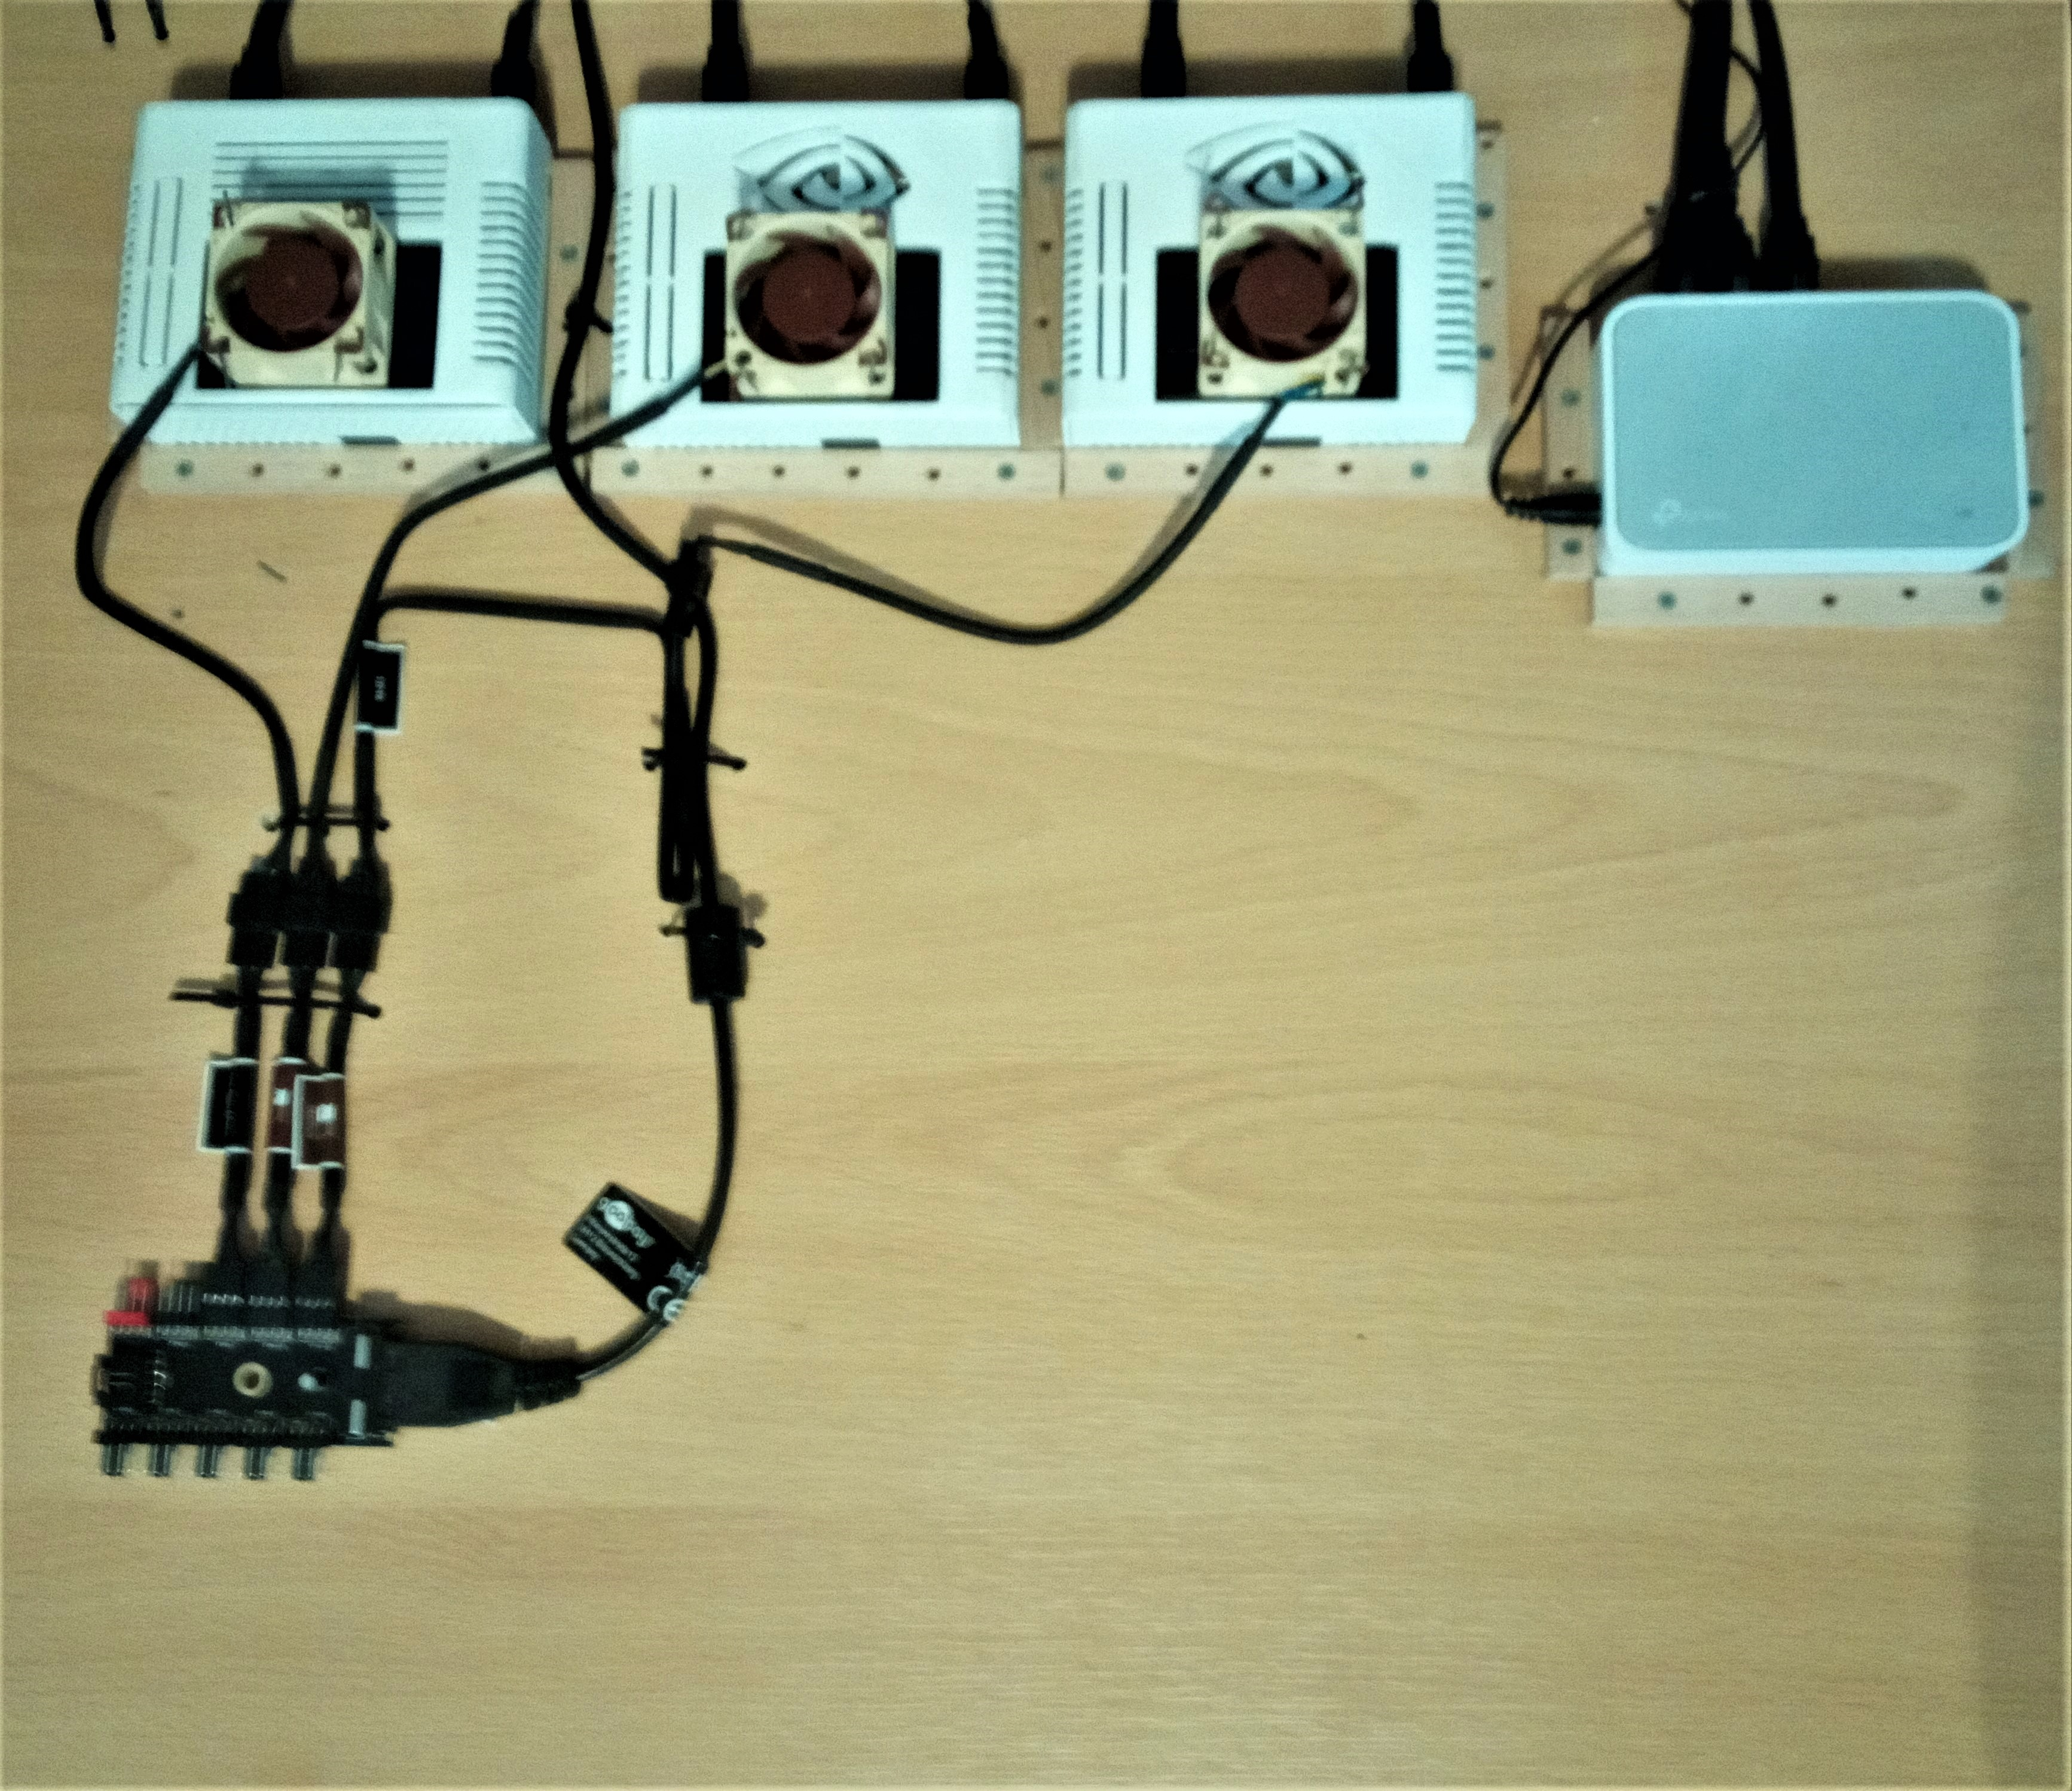
\includegraphics[width=1.0\textwidth]{images/Foto1.jpg}
	\caption{Der im Rahmen dieses Projektes erstellte Mini-Cluster. Zur besseren Nutzung wurden sowohl die Nvidia Jetson Nanos als auch der Switch durch seitliche Leisten auf einem Holzbrett fixiert. Um die vollständige Leistung durch die Nutzung des Powermodus zu erzielen, wurde desweiteren auf jedem Jetson Nano ein 40mm Lüfter installiert. Für die Steuerung dieser Lüfter wurde ein externer Lüfter-Controller genutzt, weil die Lüfter eine Betriebsspannung von 12V benötigen, der Jetson Nano jedoch nur Lüfter mit 5V Betriebsspannung unterstützt.}
	\label{img:foto1}
\end{figure}
\end{appendix}
\newpage
\bibliography{literatur}{}
\addcontentsline{toc}{section}{Literatur}  
\end{document}